\section{Floating Text}
\label{sec:floating_text}

According to this video, \href{https://www.youtube.com/watch?v=3gAlT9OWINg8}{Floating Text in Minecraft}, we need to identify the block that the armor stand will be standing on. The armor stand will always generate at the bottom of the block. (Note that the armor stand will generate as a floating entity, so it does not need a block to stand on.)

Look at a block, and type \mintinline{java}|/setblock| to get the coordinates of the block you're looking at. Copy those coordinates, and type:
\begin{minted}[breaklines]{mcfunction}
summon minecraft:armor_stand [the coordinates] {Marker:true, Invisible:true, CustomNameVisibile:true, CustomName:{"text": "[your text]", "color": "[your color]"}}
\end{minted}
For example, the code:
\begin{minted}[breaklines]{mcfunction}
summon minecraft:armor_stand -67 104 55 {Marker:true, Invisible:true, CustomNameVisible:true, CustomName:{"text": "You won!", "color": "yellow"}}
\end{minted}
will create something like this:
\begin{center}
    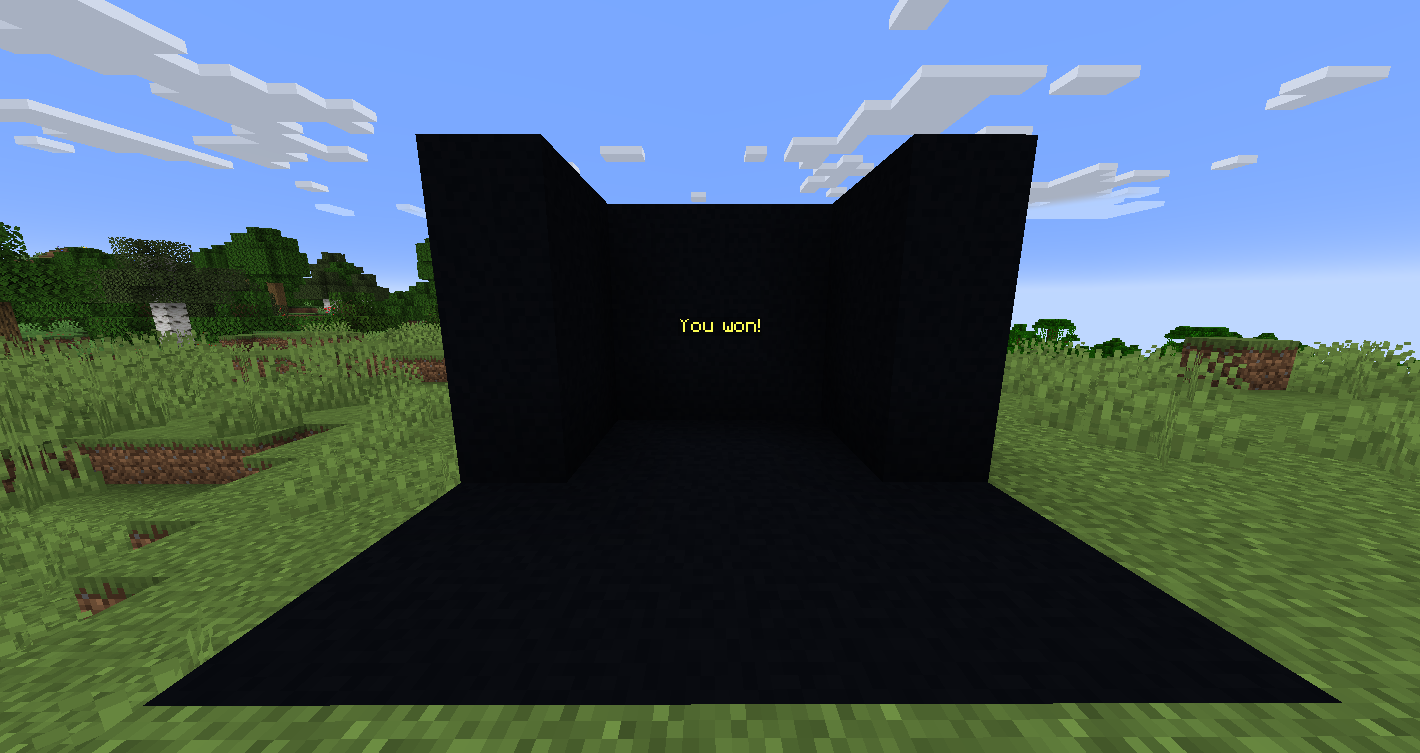
\includegraphics[width=\textwidth]{images/you_won_.png}
\end{center}

\newpage

\subsection{Adding Italics and Bold}
\label{subsec:adding_italics_and_bold}

To add italics and bold to the text, you can use the \mintinline{java}|italic| and \mintinline{java}|bold| tags. For example, the code:
\begin{minted}[breaklines]{mcfunction}
summon minecraft:armor_stand -67 104 55 {Marker:true, Invisible:true, CustomNameVisible:true, CustomName:{"text": "You won!", "color": "yellow", "italic": true, "bold": true}}
\end{minted}